\documentclass[journal]{IEEEtran}
\usepackage{graphicx,amsmath,booktabs,url}
\usepackage[hidelinks]{hyperref}
\graphicspath{{../artifacts/figures/}}
\title{Physical Action Classification from Eight-Channel Surface EMG Using Segment Statistics and k-Nearest Neighbors}
% Replace this line with your name, roll number, and course if required.
\author{Course Assignment 2 -- M2026}

\begin{document}
\maketitle
\begin{abstract}
This assignment studies the recognition of 20 physical actions from eight-channel surface electromyography (EMG). The supplied dataset contains four subjects and 80 unique recordings. Each recording is partitioned into 15 non-overlapping intervals, and each interval into three segments. Mean and sample variance features produce 1,200 observations with 48 features each. A Euclidean five-nearest-neighbor classifier is evaluated using stratified ten-fold cross-validation, with scaling estimated exclusively from the training fold. For every class count from two to 19, ten random class subsets are evaluated across ten Monte Carlo repeats. Mean accuracy decreases from 90.08\% for sampled two-class subsets to 40.51\% for 19-class subsets. A prespecified Walking--Punching case obtains 93.08\%, while the supplementary 20-class experiment obtains 39.86\%. Holding out an entire subject reduces mean accuracy to 22.33\%, showing that within-subject recording information substantially affects the trial-level results. All figures and values are computed from the supplied files; MATLAB source, an executed Python reference implementation, and reusable arrays accompany the report.
\end{abstract}
\begin{IEEEkeywords}
Surface EMG, physical actions, feature extraction, k-nearest neighbors, cross-validation, subject generalization.
\end{IEEEkeywords}

\section{Motivation and Introduction}
Surface EMG records electrical activity associated with muscle activation. Recognizing action patterns from several muscles can provide an input to human--machine interfaces, activity analysis, and assistive robotics. The supplied EMGNET presentation connects this signal-processing problem with movement assistance and discusses practical variation due to electrode placement, muscle effort, and differences between subjects~\cite{slides}. These applications motivate a classifier that is both computationally manageable and evaluated under a clearly stated prediction scenario. This experiment is an offline action-recognition study; it does not establish clinical or real-time control performance.

The supplied reference paper by Turlapaty and Gokaraju~\cite{paper} combines several time-domain, inter-channel, spectral, and local-pattern feature families. It evaluates multiple classifiers and reports 93.9\% accuracy for its selected-feature subspace kNN ensemble. The present assignment~\cite{assignment} asks a narrower question: how well do segment means and variances support kNN classification, and how does performance vary with the number of action labels? The reported paper accuracy is therefore context, not an expected or reproduced score.

The target is the identity of an action among up to 20 categories. ``Normal'' and ``Aggressive'' are directory-level groupings, not the two labels used in the binary case study. The latter distinguishes two specific activities. The workflow in Fig.~\ref{fig:pipeline} follows the assignment's four stages: data inspection, feature extraction, label construction, and repeated classification.

\begin{figure}[t]
\centering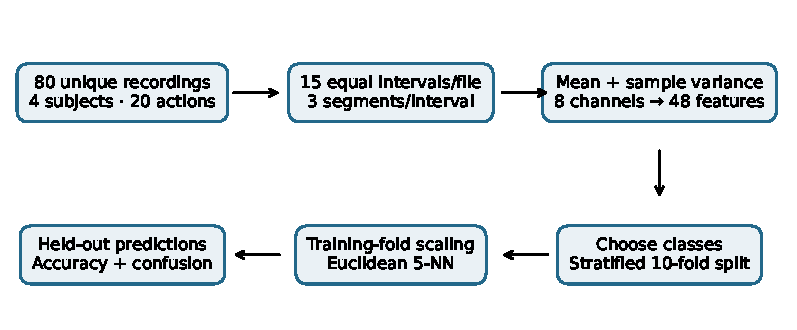
\includegraphics[width=\columnwidth]{pipeline.pdf}
\caption{Classification workflow. The scaler and kNN are fitted separately within every training fold. Class sampling and fold selection are saved for reuse.}
\label{fig:pipeline}
\end{figure}

\section{Dataset and Reproducible Data Preparation}
\subsection{Recording inventory}
The dataset readme~\cite{readme} describes four adult participants, three male and one female, performing ten normal and ten aggressive actions. Eight channels correspond to right biceps, right triceps, left biceps, left triceps, right thigh, right hamstring, left thigh, and left hamstring, in that order. Actual EMG arrays are in the \texttt{txt} directories; \texttt{log} files are intended for the acquisition software and are not additional observations.

There are four top-level subject directories, eight subject/category directories, and 80 canonical text recordings. The accidental nested directory \texttt{Data/sub3/sub3} contains 20 byte-identical copies, verified by SHA-256. These copies are excluded without changing the original files. Recursive loading without this check would incorrectly add a fifth subject copy or overweight subject 3.

\begin{table}[t]
\caption{Measured inventory of canonical recordings}
\label{tab:inventory}\centering\small
\begin{tabular}{rrrr}\toprule
Subject & Files & Rows per file & Total rows\\\midrule
1 & 20 & 9611--10000 & 197058 \\
2 & 20 & 9806--10000 & 199620 \\
3 & 20 & 9205--15106 & 204215 \\
4 & 20 & 9464--10000 & 196533 \\
\bottomrule\end{tabular}
\end{table}

Every array has eight columns; the observed row counts range from 9205 to 15106, rather than all being exactly 10,000. Across files there are 797,426 multichannel time samples. The complete file list, shapes, ranges, and hashes are exported to \texttt{artifacts/dataset\_manifest.csv}. Table~\ref{tab:inventory} summarizes these checks. Data are validated as numeric and finite. No recording is removed based on its classification performance.

\begin{table}[t]
\caption{Deterministic labels: alphabetical within each category}
\label{tab:labels}\centering\small
\begin{tabular}{rlrl}\toprule
ID & Normal action & ID & Aggressive action\\\midrule
1 & Bowing & 11 & Elbowing \\
2 & Clapping & 12 & Frontkicking \\
3 & Handshaking & 13 & Hamering \\
4 & Hugging & 14 & Headering \\
5 & Jumping & 15 & Kneeing \\
6 & Running & 16 & Pulling \\
7 & Seating & 17 & Punching \\
8 & Standing & 18 & Pushing \\
9 & Walking & 19 & Sidekicking \\
10 & Waving & 20 & Slapping \\
\bottomrule\end{tabular}
\end{table}

Label assignment uses the sorted file count in each category: Normal receives 1--10 and Aggressive receives 11--20. The same filename order is checked for all subjects. Table~\ref{tab:labels} preserves dataset spellings, including ``Hamering'' and ``Headering.'' Each label has exactly $4\times15=60$ observations.

\subsection{Raw signal inspection and preprocessing decisions}
Fig.~\ref{fig:raw} displays all eight channels for one normal action and one aggressive action from subject 1. Horizontal axes use sample indices because the text arrays and readme do not specify a calibrated time axis for every recording. Vertical values are retained in the units stored in the files; a voltage conversion is not invented.

The readme explicitly states that subject 2 is unfiltered. The files also contain large offsets and values at magnitude 4,000. The manifest records the proportion with $|x|\geq4,000$ as a descriptive data-quality indicator; it does not prove a particular hardware saturation threshold. No additional band-pass filter, rectification, or per-recording normalization is imposed. This keeps the required mean/variance baseline explicit and preserves the original data, while leaving preprocessing differences as a limitation. Feature scaling within training folds addresses feature units, not acquisition inconsistencies.

\begin{figure}[t]
\centering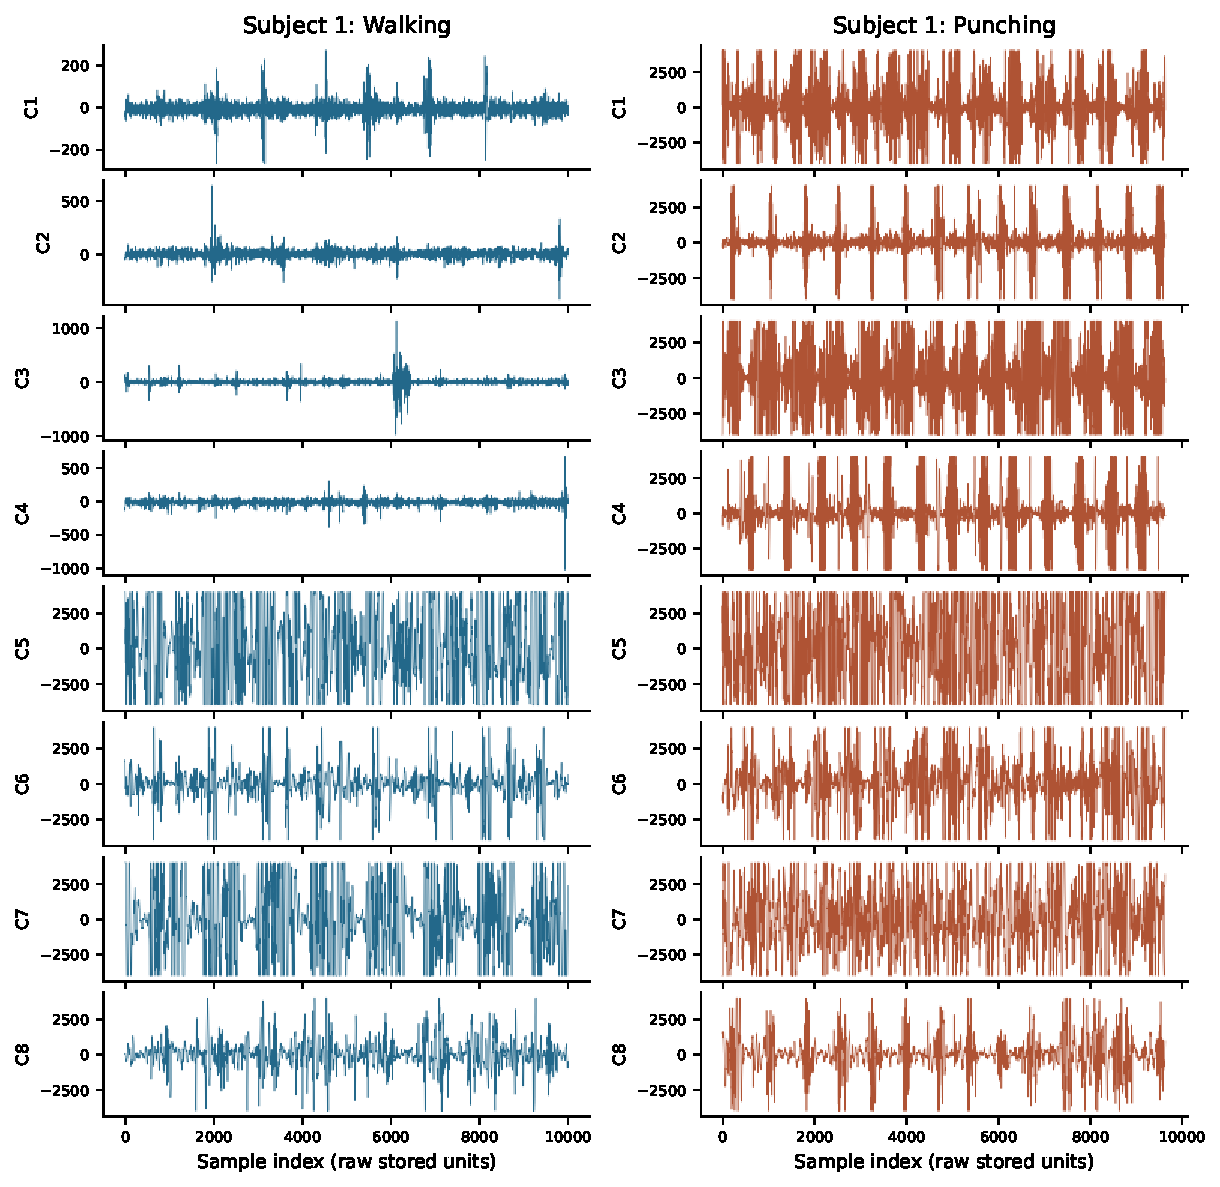
\includegraphics[width=\columnwidth]{raw_signals.pdf}
\caption{All eight raw channels for subject 1: Walking (Normal, label 9) and Punching (Aggressive, label 17). Each panel has its own amplitude scale.}
\label{fig:raw}
\end{figure}

\section{Feature Construction and Classifier}
\subsection{Trial and segment boundaries}
For a file with $L$ rows, the zero-based boundaries of its 15 intervals are
\begin{equation}
b_t=\left\lfloor\frac{tL}{15}\right\rfloor,\qquad t=0,\ldots,15.
\end{equation}
Interval $t$ contains indices $b_{t-1},\ldots,b_t-1$. Its length $L_t$ is divided into $N_{\mathrm{seg}}=3$ segments using boundaries $\lfloor sL_t/3\rfloor$ for $s=0,1,2,3$. This rule uses every sample exactly once, introduces no overlap, and gives segment lengths differing by at most one. Interval lengths range from 613 to 1008 samples in these files.

The assignment specifies 15 trials per array but supplies no onset/offset annotations. Equal intervals are therefore an operational approximation to trials, not verified movement-aligned repetitions. The reference paper uses approximately 666 samples per trial for nominally 10,000-sample records~\cite{paper}. Using each file's actual length avoids silently truncating the longer records. Three segments are fixed before evaluation to retain coarse temporal order while keeping the feature vector small. This setting is not selected by maximizing test accuracy, and no claim of optimality is made.

\subsection{Mean and sample variance}
For channel $c$ and segment $s$ with $n_s$ samples, the two required statistics are
\begin{align}
\mu_{c,s}&=\frac{1}{n_s}\sum_{i=1}^{n_s}x_{c,s,i},\\
v_{c,s}&=\frac{1}{n_s-1}\sum_{i=1}^{n_s}(x_{c,s,i}-\mu_{c,s})^2.
\end{align}
The variance uses the sample convention, matching MATLAB's \texttt{var(x,0)} and NumPy's \texttt{ddof=1}. All features from one interval remain in one observation. Feature order is channel, then segment, then statistic: $[\mu_{1,1},v_{1,1},\mu_{1,2},v_{1,2},\ldots,\mu_{8,3},v_{8,3}]$. The resulting dimensions are
\begin{align}
N_f&=8\times3\times2=48,\\
N&=4\times20\times15=1200.
\end{align}
The MATLAB array \texttt{X} is $1200\times48$, \texttt{y} is $1200\times1$, and the concatenated \texttt{data=[X y]} is $1200\times49$. Subject and interval identifiers are saved alongside them. A two-class subset is $120\times48$, with a $120\times1$ target vector. The arrays are available in both \texttt{.mat} and \texttt{.npz} formats.

\begin{figure}[t]
\centering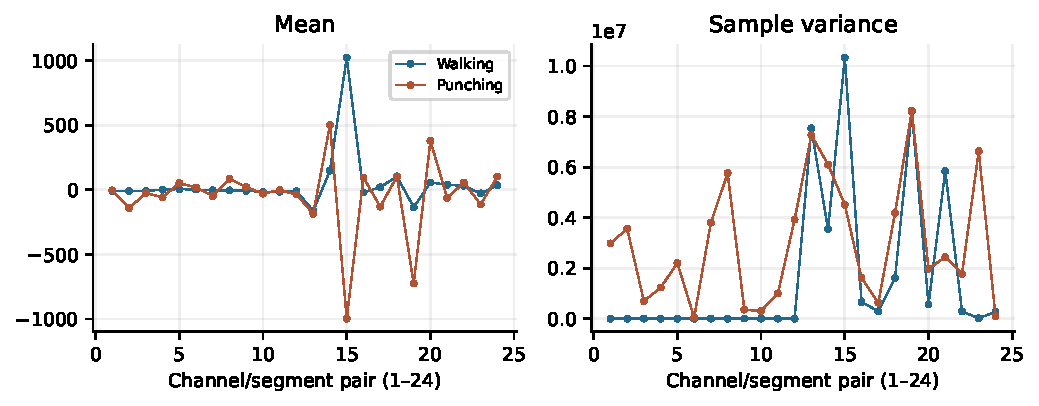
\includegraphics[width=\columnwidth]{example_features.pdf}
\caption{Actual feature vectors from the first interval of subject 1's Walking and Punching files. Mean and variance are shown separately because their units and scales differ. All 48 values are listed in the accompanying example-features CSV.}
\label{fig:features}
\end{figure}

Means retain local offsets and average signal level; variances represent local dispersion. These statistics compress the waveform substantially and discard detailed temporal and frequency structure. Fig.~\ref{fig:features} visualizes the two statistics for the selected binary case, without using the plot as a feature-selection step.

\subsection{Scaling and Euclidean kNN}
For feature $j$, the training-fold mean $a_j$ and sample standard deviation $d_j$ define $z_j=(f_j-a_j)/d_j$. A zero training standard deviation is replaced by one. The test fold is transformed using the training values only. This prevents test data from influencing the metric and prevents variance features from dominating merely because of their numeric scale.

The classifier uses $k=5$ neighbors, Euclidean distance, and uniform majority voting. Voting ties are resolved by the smallest numeric class label. Python uses scikit-learn's exact brute-force implementation, while the supplied MATLAB code implements the same rule using distances, sorting, and \texttt{mode}; a Statistics Toolbox is not required. Exact distance ties at the fifth-neighbor boundary can produce small implementation differences. Neither $k$ nor the feature settings are tuned on the evaluation folds.

\section{Experimental Protocol}
\subsection{Cross-validation and Monte Carlo design}
The main evaluation uses stratified ten-fold cross-validation. Each class contributes six test observations in each fold; the other 54 are used for training. Out-of-fold predictions cover each observation exactly once per repeat. Accuracy is the proportion correctly predicted over these held-out predictions. Ten Monte Carlo repeats vary the fold assignments, and random seeds are fixed from master seed 2026.

For each $M\in\{2,3,\ldots,19\}$, all $\binom{20}{M}$ label combinations are enumerated in lexicographic order. Ten uniformly random combination ranks are drawn \emph{with replacement}, following the handout's \texttt{randi} instruction. Those ten subsets are held fixed across the ten fold repeats for that $M$. Duplicate draws, if any, are retained as part of the specified sampling design. The largest combination list has $\binom{20}{10}=184,756$ entries and is discarded after its selections are recorded.

Let $A_{M,c,r}$ denote accuracy for class count $M$, sampled combination $c$, and repeat $r$. The stored accuracy tensor is $18\times10\times10$, or 1,800 cross-validation results and 18,000 individual model fits. The heatmap plots
\begin{equation}
H_{M,r}=\frac{1}{10}\sum_{c=1}^{10} A_{M,c,r},
\end{equation}
and the class-count curve plots
\begin{equation}
\overline A_M=\frac{1}{100}\sum_{c=1}^{10}\sum_{r=1}^{10} A_{M,c,r}.
\end{equation}
Thus every point averages over both sources of repetition, rather than treating only one selected combination as representative of a class count. The saved plan contains selected labels, one-based ranks, and every fold assignment. Repeats reuse the same observations and are not independent replications of data collection.

\subsection{Binary, full-class, and subject-held-out checks}
Walking (9) versus Punching (17) is fixed as the binary case before inspecting its performance. This gives 120 observations, 60 per action. It uses the same feature construction and ten repeated ten-fold evaluations. Macro F1 and a confusion matrix complement accuracy.

A supplementary 20-class experiment includes all 1,200 observations under the same repeated protocol. Finally, leave-one-subject-out (LOSO) evaluation trains on three complete subjects and tests on the fourth, giving four folds with 900 training and 300 test observations each. Scaling is refitted within each LOSO fold. This stricter test addresses an unseen-subject scenario; the required shuffled trial-level experiment can place intervals from the same recording in both training and test sets.

\subsection{Criterion for rapid degradation}
An adjacent loss $D_M=\overline A_M-\overline A_{M+1}$ of at least 0.05 (five percentage points) is used as an explicit descriptive ``rapid-drop'' rule. The largest adjacent loss is also reported. This rule is not a statistical change-point test. Because different subsets are sampled at each $M$, an adjacent loss mixes class-count effects and subset composition. A universal critical number of classes cannot be inferred from one small dataset.

\section{Results and Case Studies}
\subsection{Binary classification}
Walking versus Punching obtains mean accuracy 93.08\% with a repeat-to-repeat standard deviation of 1.71 percentage points and mean macro F1 of 0.931. Its balanced chance accuracy is 50\%. Fig.~\ref{fig:binary} pools the ten out-of-fold confusion matrices. Each action contributes 600 predictions, but there are only 60 unique observations per action; the repeated counts must not be interpreted as 1,200 independent binary samples. There are 83 errors among the 1,200 repeated predictions.

\begin{figure}[t]
\centering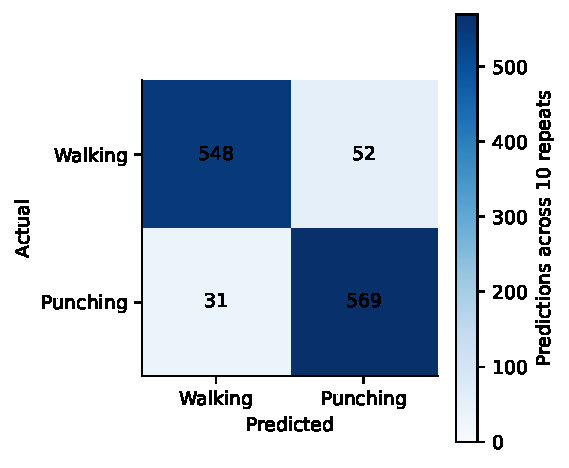
\includegraphics[width=.88\columnwidth]{binary_confusion.pdf}
\caption{Walking--Punching confusion matrix pooled over ten cross-validation repeats. Counts summarize repeated predictions of the same 120 observations.}
\label{fig:binary}
\end{figure}

The selected pair's accuracy and the mean across ten randomly sampled pairs answer different questions. The former concerns one fixed pair of activities, while the latter averages several action-separation problems of varying difficulty. Neither score alone establishes performance for the full action vocabulary or for a new user.

\subsection{Accuracy as the number of classes increases}
Table~\ref{tab:curve} and Fig.~\ref{fig:curve} report the requested $M=2$--19 results. The sampled two-class mean is 90.08\%, decreasing to 40.51\% for 19 classes. Balanced chance is $1/M$, so changing the number of classes changes both the decision problem and its chance level. The shaded range is one sample standard deviation across the ten subset means; it describes subset sensitivity and is not a confidence interval.

\begin{table}[t]
\caption{Measured accuracy versus class count. All values are percentages or percentage points. SD$_c$: SD of ten subset means; SD$_r$: SD of ten repeat means.}
\label{tab:curve}\centering\small
\begin{tabular}{rrrr}\toprule
$M$ & Mean accuracy & SD$_c$ & SD$_r$\\\midrule
2 & 90.08 & 6.41 & 0.21 \\
3 & 75.93 & 8.87 & 0.61 \\
4 & 69.80 & 7.80 & 0.45 \\
5 & 69.26 & 7.52 & 0.36 \\
6 & 63.40 & 6.21 & 0.31 \\
7 & 58.17 & 2.52 & 0.28 \\
8 & 57.42 & 5.69 & 0.35 \\
9 & 54.76 & 4.93 & 0.24 \\
10 & 53.37 & 5.26 & 0.39 \\
11 & 53.45 & 3.28 & 0.33 \\
12 & 49.98 & 1.39 & 0.25 \\
13 & 48.62 & 2.47 & 0.24 \\
14 & 47.51 & 2.47 & 0.23 \\
15 & 45.19 & 2.29 & 0.25 \\
16 & 43.45 & 2.10 & 0.30 \\
17 & 43.35 & 1.20 & 0.16 \\
18 & 42.10 & 0.75 & 0.29 \\
19 & 40.51 & 0.90 & 0.25 \\
\bottomrule\end{tabular}
\end{table}

\begin{figure}[t]
\centering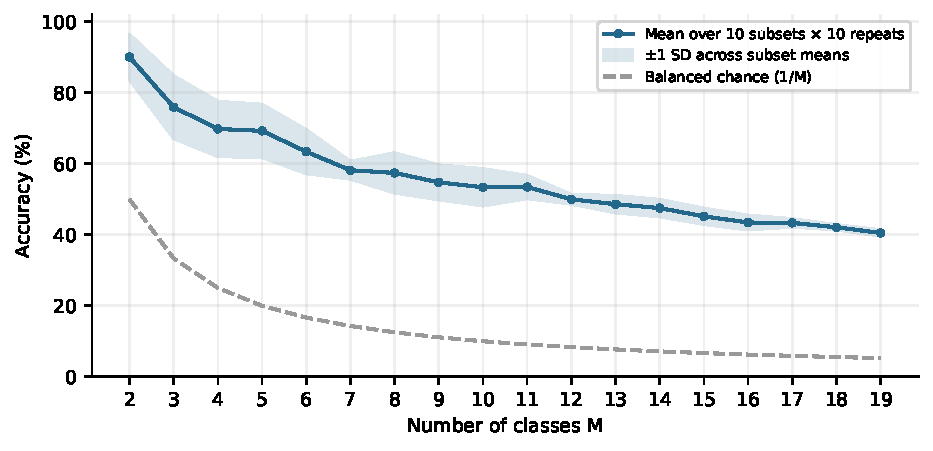
\includegraphics[width=\columnwidth]{accuracy_vs_classes.pdf}
\caption{Mean accuracy across sampled class combinations and Monte Carlo repeats. Shading shows $\pm1$ SD across subset means, not uncertainty for independent subjects. The dashed line is balanced chance.}
\label{fig:curve}
\end{figure}

The largest adjacent decrease is 14.15 percentage points, from $M=2$ to $M=3$. The first transition meeting this rule is $M=2$ to $M=3$. The conclusion is an operational description of this particular sampled curve, rather than evidence that all EMG classifiers fail after that many categories. Non-monotone points are possible because the subsets at successive class counts are different and do not form a nested sequence.

\begin{figure}[t]
\centering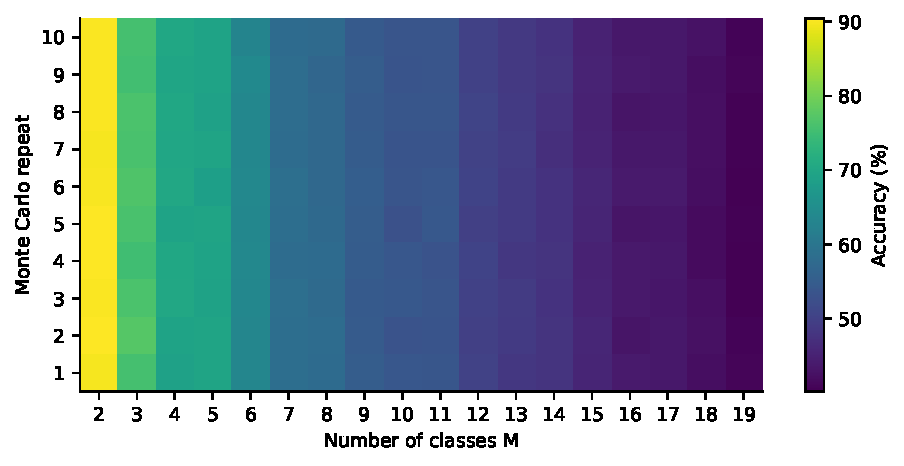
\includegraphics[width=\columnwidth]{mc_heatmap.pdf}
\caption{Required accuracy heatmap: number of classes versus Monte Carlo repeat. Each cell averages the ten selected class combinations at that class count.}
\label{fig:heatmap}
\end{figure}

Fig.~\ref{fig:heatmap} displays fold-repeat sensitivity at each class count. The two SD columns in Table~\ref{tab:curve} distinguish variation due to selected actions from variation after averaging over actions within a repeat. Since all repeats share data and all subsets draw from the same 20 labels, these dispersions should not be interpreted as population-level confidence bounds.

\subsection{All 20 classes and error structure}
With every class included, accuracy is 39.86\% $\pm$ 0.59 percentage points across repeats, and mean macro F1 is 0.385. Fig.~\ref{fig:multi} shows row-normalized recalls from the pooled confusion matrix; each row has 600 predictions of 60 distinct observations. Chance accuracy is 5\%. Table~\ref{tab:confusions} lists the five largest directional off-diagonal counts, making the dominant errors directly inspectable.

\begin{figure}[t]
\centering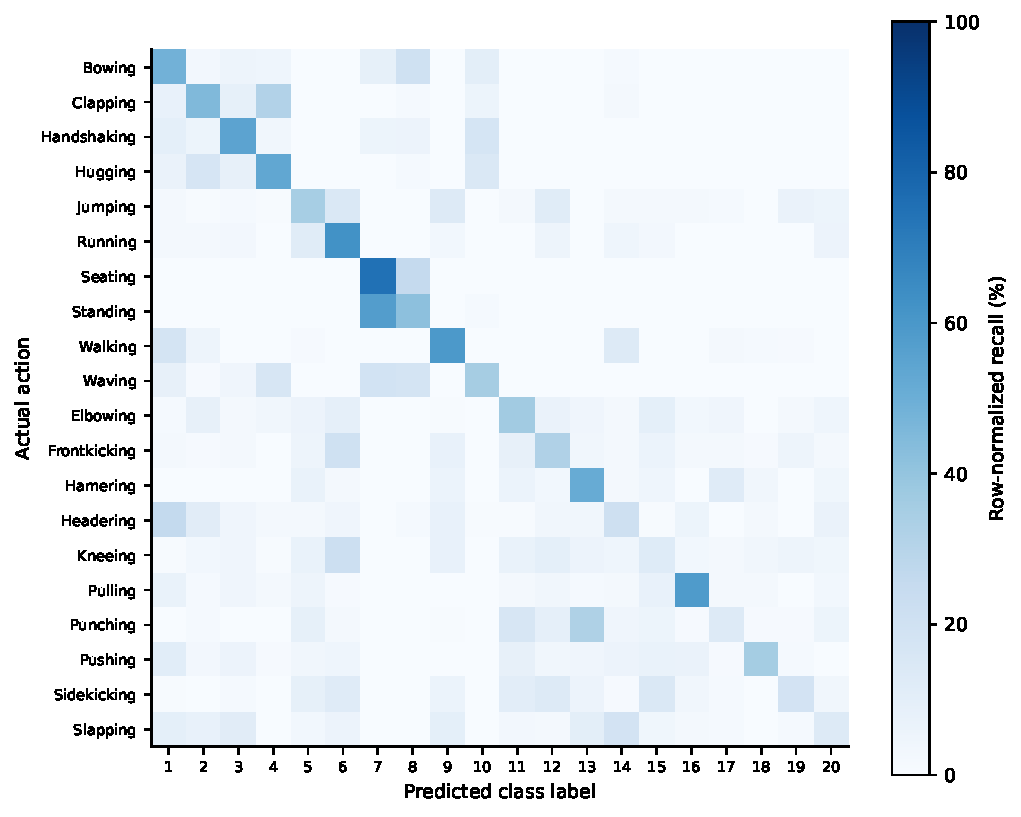
\includegraphics[width=\columnwidth]{multiclass_confusion.pdf}
\caption{Supplementary 20-class confusion matrix, normalized within actual class. Horizontal labels refer to Table~\ref{tab:labels}. Aggregation is over all ten repeats.}
\label{fig:multi}
\end{figure}

\begin{table}[t]
\caption{Largest directional confusions in the 20-class experiment}
\label{tab:confusions}\centering\small
\begin{tabular}{llr}\toprule
Actual & Predicted & Count / 600\\\midrule
Standing & Seating & 343 \\
Punching & Hamering & 194 \\
Clapping & Hugging & 187 \\
Headering & Bowing & 154 \\
Seating & Standing & 152 \\
\bottomrule\end{tabular}
\end{table}

These errors show which action labels overlap in the chosen statistical representation. Means and variances may summarize distinct waveforms similarly, and acquisition differences may shift otherwise similar actions apart. The results do not isolate a physiological cause for a particular confusion. Richer spectral and inter-channel features, as studied in the reference paper, are possible future extensions; they have not been substituted for the assignment's prescribed features here.

\subsection{Generalization to unseen subjects}
LOSO accuracy is 22.33\% averaged over four equally sized held-out subjects. The individual scores for subjects 1--4 are 24.33\%, 12.33\%, 31.00\%, 21.67\%. Fig.~\ref{fig:loso} reports each fold. The difference from shuffled trial-level accuracy is material: holding out a person removes subject-specific examples and the shared recording context from the training data.

\begin{figure}[t]
\centering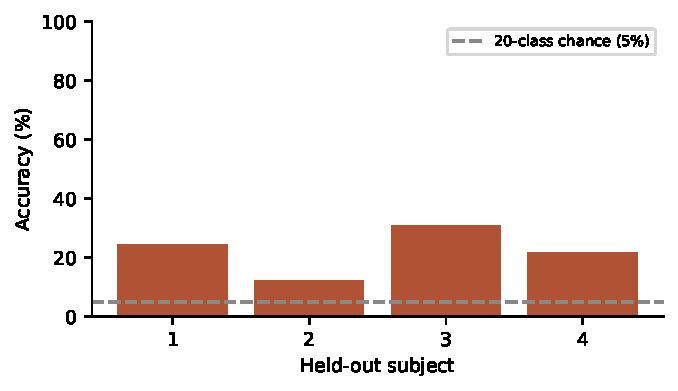
\includegraphics[width=\columnwidth]{subject_holdout.pdf}
\caption{Twenty-class leave-one-subject-out accuracy. Each test fold contains 300 intervals from one person; the dashed line marks 5\% chance.}
\label{fig:loso}
\end{figure}

\section{Limitations, Verification, and Reproducibility}
\subsection{Interpretation limits}
There are four participants, not 1,200 independent participants. Equal interval boundaries may cut across true action repetitions, and nearby intervals can remain correlated. Trial-level cross-validation estimates recognition of new intervals from the represented subject/recording mixture; it is not a subject-independent estimate. The supplementary LOSO result directly exposes this distinction, but four subjects are still too few for broad population conclusions.

Subject 2's unfiltered acquisition, offsets, possible clipping, and variable recording length are retained. The analysis does not measure whether any one of these factors causes a particular error. A future study could collect annotated repetitions, apply a documented common acquisition/filtering protocol, and select feature settings inside nested subject-grouped validation. Such extensions would require additional experiments and are not presented as completed results.

Only ten sampled combinations are evaluated at each class count, as requested; this is not an exhaustive performance evaluation over all combinations. Mean and variance retain limited information. Repeating folds reduces sensitivity to a particular split but cannot create additional independent people or sessions. No comparison with the reference paper is a controlled ablation because feature families, classifier design, and protocol details differ.

\subsection{Execution environment and resource control}
All reported numerical experiments were executed using Python 3.9.6, NumPy 2.0.2, SciPy 1.13.1, and scikit-learn 1.6.1 on macOS ARM64. The user identified the machine as a MacBook Air M5. The run uses one numerical-library thread and one kNN worker, no GPU, a 0.05-second pause after each cross-validation evaluation, and a one-second pause after each group of ten evaluations. Completed class-count batches are checkpointed with a fingerprint of inputs, configuration, code, and scikit-learn version. These settings limit concurrent work; they are not a temperature guarantee. Thermal telemetry was unavailable through the execution sandbox.

MATLAB is not installed in the execution environment. The MATLAB implementation is supplied for all tasks but its runtime has not been verified here. It can load the exact exported combinations and folds, and it checks feature agreement against the executed Python arrays before classification. Without the exported plan it can generate its own seeded combinations and stratified folds, whose random numbers will differ from Python. The reported scores are explicitly the executed Python results, not claimed MATLAB output.

Automated checks verify exhaustive non-overlapping segmentation, known hand-computed mean/variance values and feature order, training-only scaling under an extreme test outlier, stratified fold sizes, the saved $1200\times48$ matrix, and exclusion of nested duplicates. The final result files and figures are derived from out-of-fold predictions or the stored accuracy tensor. Source code and data are linked below so that these checks and results can be repeated.

\section{Conclusion}
The required pipeline converts the supplied eight-channel recordings into 1,200 labeled observations with 48 segment-statistic features. The Walking--Punching case reaches 93.08\%, whereas the complete 20-action problem reaches 39.86\% under repeated trial-level cross-validation. Across sampled subsets, the largest adjacent loss occurs from 2 to 3 classes. The markedly different LOSO accuracy of 22.33\% cautions against interpreting shuffled interval performance as recognition for unseen subjects. The delivered arrays, split plan, MATLAB implementation, executed Python analysis, and figures provide a reproducible baseline for the assignment's prescribed method.

\section*{Code and Data Availability}
The accompanying repository is the source package for this report. Relative links below work when the report remains in the \texttt{report} directory and the PDF viewer permits local file links. The same paths are written explicitly for viewers that block such links.
\begin{itemize}
\item MATLAB entry point: \href{run:../matlab/run_assignment.m}{\texttt{matlab/run\_assignment.m}}; feature extractor: \href{run:../matlab/extract_trial_features.m}{\texttt{matlab/extract\_trial\_features.m}}.
\item Executed analysis: \href{run:../src/emg_assignment.py}{\texttt{src/emg\_assignment.py}}; settings: \href{run:../config.json}{\texttt{config.json}}; run commands: \href{run:../README.md}{\texttt{README.md}}.
\item Arrays: \href{run:../artifacts/emg_features.mat}{\texttt{artifacts/emg\_features.mat}}; exact selections and folds: \href{run:../artifacts/experiment_plan.mat}{\texttt{artifacts/experiment\_plan.mat}}.
\item Numerical results: \texttt{artifacts/results/}; figures: \texttt{artifacts/figures/}; tests: \texttt{tests/test\_pipeline.py}.
\end{itemize}
The code is linked instead of reproduced as a long appendix, as permitted by the assignment. The submission ZIP includes these paths and the input recordings.

\begin{thebibliography}{5}
\bibitem{slides} A. C. Turlapaty \emph{et al.}, ``EMGNET,'' WADLA 2021, IIIT Sri City, workshop presentation. Supplied file: \texttt{EMGNET-V2\_2.pdf}, especially slides 39--44 and 51--55.
\bibitem{paper} A. C. Turlapaty and B. Gokaraju, ``Feature analysis for classification of physical actions using surface EMG data,'' \emph{IEEE Sensors Journal}, vol. 19, no. 24, pp. 12196--12204, Dec. 2019, doi: \href{https://doi.org/10.1109/JSEN.2019.2937979}{10.1109/JSEN.2019.2937979}.
\bibitem{assignment} ``Analysis of physical actions,'' CA2--M2026, supplied two-page assignment handout, \texttt{CA2 - M2026 - EMG Signal Classification.pdf}.
\bibitem{readme} T. Theodoridis, ``EMG Physical Action DataSet,'' University of Essex, dataset readme, July 28, 2011. Supplied file: \texttt{Data/readme.txt}.
\bibitem{template} M. Shell, ``IEEEtran: Document class for IEEE journals and conferences,'' CTAN. [Online]. Available: \url{https://ctan.org/pkg/ieeetran}. Used in journal mode for this report.
\end{thebibliography}
\end{document}
